%----------------------------------------------------------------------------
\chapter{Android alkalmazás beszélőfelismerésre}
%----------------------------------------------------------------------------

A következő fejezetben bemutatom egy általam a beszélőfelismerés szemléltetésére készített android alkalmazás fő elemeit és működését, a kapcsolódó technológiákat és implementációs részleteket. Az alkalmazásban konkrét beszélőfelismerésre készített neurális hálózatokat használok fel. A cél nem egy új beszélőfelismerő modell készítése volt, hanem az eddigiek felhasználásával egy működő alkalmazás létrehozása.

Az alkalmazás kliens-szerver architektúrájú lesz. Az android kliens segítségével a felhasználó regisztrálhat a rendszerbe névvel és hanggal, majd az azonosítás opció megnyomásával hangmintát adva az alkalmazás eldönti, hogy regisztrálva van-e, és ha igen, akkor visszaadja az illető nevét.

\section{Modell predikció a felhőben vagy lokálisan?}


A szervernek tárolnia kell a felhasználóktól származó hangmintákat és a felhasználó azonosítás folyamata közben összehasonlítani őket. Az összehasonlítást egy sziámi neurális hálózat végzi. Az alkalmazás felépítését tekintve a legfontosabb kérdés, hogy ezt az összehasonlítást központilag egy felhőben a szerver, vagy a kliens oldali alkalmazás végezze. Mivel a modell végzi a predikciót, ettől a döntéstől függően azt a szerveren vagy a kliens eszközökön kell tárolni. Mindkét architektúrának vannak előnyei és hátrányai is.

Mivel esetünkben az alkalmazás kész, előre tanított modelleket használ, nincs szükség a modellek tanítására. Ennek ellenére ha a jövőben saját modellt szeretnénk használni felmerül a kérdés, hogy hol tanítsuk azt.

\begin{itemize}
	\item A felhőben hosztolt gépi tanulási szolgáltatások általában saját modelleket használnak. Mi a saját adatainkat átadjuk és a szolgáltatás gondoskodik a modell tanításáról. Ezután a predikciót egy API-n keresztül végezhetjük el. Figyelni kell arra, hogy ebben az esetben nem mindig miénk a modell. Ha nincs lehetőség tanítás után a modell letöltésére, akkor a predikció mindenképp a felhőben marad. Másrészről a magas szintű szolgáltatások kezelése könnyebb, nem kell érteni a neurális hálózatok tanításához, de nem elég flexibilisek. Általában nem változtathatunk a modellen és az API-n sem.
	
	\item A felhőben taníthatjuk a modellünket az erre készített szolgáltatások nélkül is nagyobb hozzáértést feltételezve. Ekkor megválaszthatjuk a modell típusát és a technológiákat (Tensorflow, Pytorch, stb.) és teljes mértékben miénk a modell és az irányítás. A lokális tanítással szemben további előny, hogy az erőforrásokat rugalmasan fel-le skálázhatjuk.
	
	\item Lokálisan is taníthatjuk a modellt. Ez főleg akkor éri meg, ha van elég erőforrásunk hozzá vagy a modell mérete nem indokolja több erőforrás használatát. Nagyobb modellek esetében a tanítási idő hosszú. Az árakat és az időt mérlegelve dönteni kell, hogy a lehetőségek közül melyiket indokolt választani.
\end{itemize}

Ha már rendelkezünk egy működő modellel, akkor el kell döntenünk, hogy a predikciót a felhőben vagy lokálisan az eszközön végezzük.

\begin{itemize}
	\item A hálózati kapcsolatot tekintve ha a predikciót lokálisan végezzük, nincs szükség internetkapcsolatra, predikció a készüléken történik. Ellenkező esetben a kliens interneten keresztül kérést küldd a szervernek, ami elvégzi a predikciót és visszaküldi a választ.
	\item A modellt felhőben a szerveren tárolni biztonságosabb. Lokális predikció esetén a modellt a készüléken tároljuk. Ilyenkor gondoskodni kell a biztonságáról, hogy ne lehessen visszafejteni azt (reverse engineering).
	\item A predikció sebessége is meghatározó szempont. Ha lokálisan, a mobiltelefon hatja végre, a felhőhöz képest kisebb erőforrással gazdálkodunk, ami miatt lassabb lesz a számítás. Viszont ha a felhőben végezzük, a kommunikációs overhead hozzáadódik a válaszhoz. Le kell mérni, hogy a kliens-szerver kommunikáció késleltetése mekkora az erőforráskülönbségből származó számítási időkhöz képest.
	\item Az alkalmazás architektúráját tekintve ha a modell és a predikció a szerveren történik, bármikor frissíthetjük, finomhangolhatjuk a modellt és ehhez nem kell a felhasználóknak frissítéseket letölteniük. Nincs szükség szinkronizációra. Az alkalmazás elosztott, elkülönült backend és frontend részekből áll, amelyek egy interfészen keresztül kommunikálnak, így ezek a komponensek lecserélhetők, csak az interfészt kell implementálniuk (API).
	\item Felhőbeli erőforrásokat használva az árat is figyelembe kell venni. Minél több felhasználó használ egy alkalmazást és amennyiben a számítás központilag a felhőben történik, annál több erőforrásra van szükség. Nagy előnye a készüléken végzett predikciónak, hogy jól skálázódik. Több felhasználó esetén nincs szükség több erőforrásra.
\end{itemize}

Jelen alkalmazás egy beszélőfelismerő szoftvert szemléltet, amelyet a valóságban vállalatok üzemeltetnek beléptető kapuval biometrikus azonosításként. Központi szerverre szükség van a regisztrált felhasználók adatainak biztonságos tárolása és a könnyű szinkronizáció miatt. Ha feltesszük, hogy a beléptető rendszert nem több mint tízezer ember azonosítására használják és a belépés szekvenciálisan történik, óriási erőforrásokat sem kell használni, mert a szerver egy időben legfeljebb a beléptető kapuk száma szerinti számítást kell végezzen, ami korlátos. Ezeket figyelembe véve úgy döntöttem, hogy a modell tárolása és a predikció szerveren fog történni.

\section{Alkalmazás architektúra és általános működés}

Mivel az alkalmazás tárolja a regisztrált felhasználók hangmintáit és a modellt; a biztonság, a könnyű központi adminisztráció és hogy nincs szükség szinkronizációra mind megerősíti a kliens-szerver architektúra szükségességét és előnyeit, így peer-to-peer megoldás fel sem merült.

\begin{figure}[!ht]
	\centering
	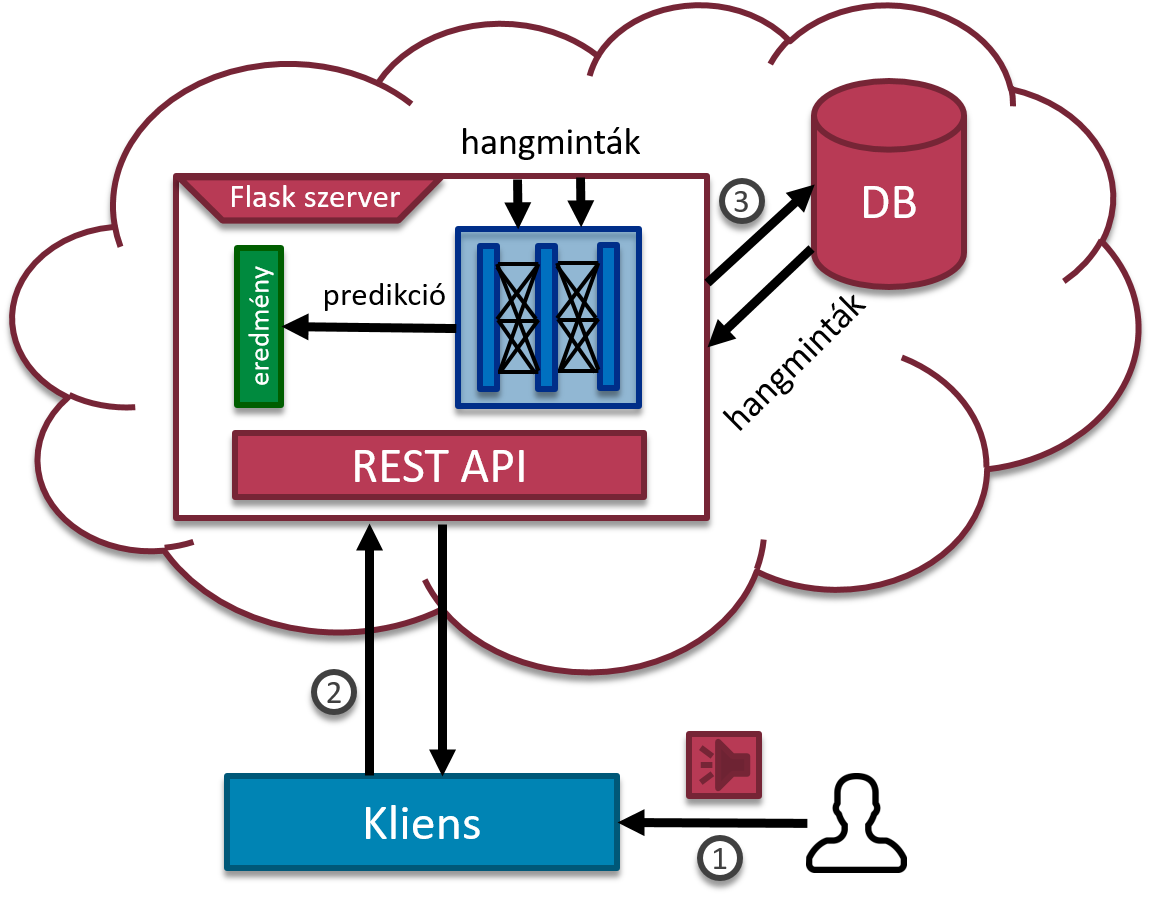
\includegraphics[width=100mm, keepaspectratio]{figures/app-register.png}
	\caption{Beszélőfelismerő alkalmazás: Regisztrációs fázis.}
	\label{fig:app-register}
\end{figure}

A \ref{fig:app-register} ábrán látható kliens a felhőben futó szerverrel egy REST API-n keresztül kommunikál. A kliens segítségével a felhasználó regisztrál a rendszerbe, ezután azonosíthatja magát. A regisztrációs fázis működése a következő:

\begin{enumerate}
	\item A felhasználó hangját és nevét a kliens alkalmazás rögzíti.
	\item A kliens a hangmintát és a nevet elküldi a szervernek a REST API-n keresztül.
	\item A szerver előfeldolgozza a hangfájlt, majd menti a névvel együtt az adatbázisba.
\end{enumerate}

Miután a felhasználók regisztráltak, az alkalmazás a hangjuk alapján azonosítani tudja őket. Az azonosítási fázis lépéseit a \ref{fig:app-identify} ábra mutatja.

\begin{figure}[!ht]
	\centering
	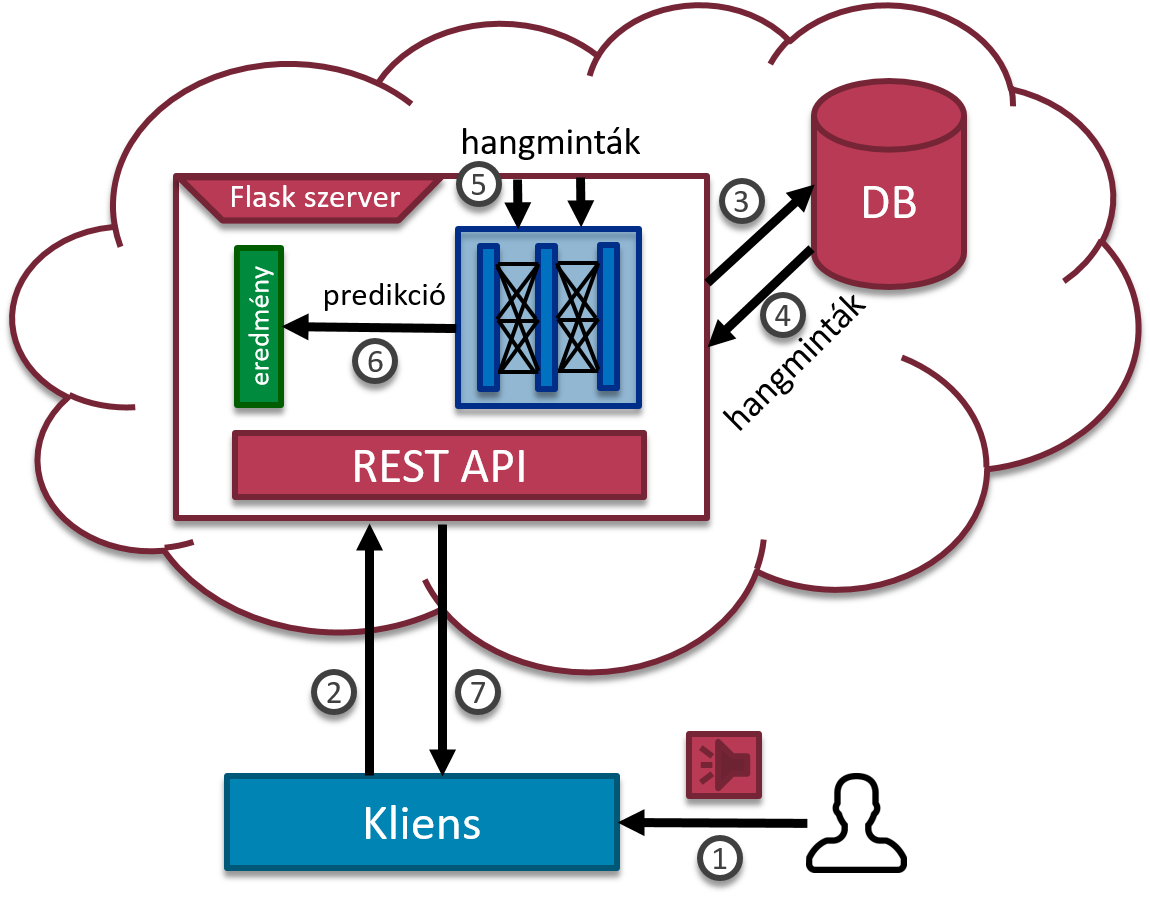
\includegraphics[width=100mm, keepaspectratio]{figures/app-identify.png}
	\caption{Beszélőfelismerő alkalmazás: Regisztrációs fázis.}
	\label{fig:app-identify}
\end{figure}

\begin{enumerate}
	\item A kliens rögzíti az azonosítani kívánt felhasználó hangját.
	\item A hangmintát továbbítja a szervernek.
	\item A szerveren futó alkalmazás a hangfájlt előfeldolgozza és eltárolja.
	\item A hangmintákat az adatbázisból betölti és azonosítandó - nem azonosítandó párokat készít belőle.
	\item A hangminta párokat a modell bemenetére adja.
	\item A modell kiszámolja a hangminták közötti hasonlósági pontokat. Ezután az alkalmazás a hasonlósági küszöbszámot figyelembe véve dönt arról, hogy azonosítható-e a felhasználó.
	\item A szerver válaszol az azonosított felhasználó nevével, vagy közli, hogy a felhasználó nincs a rendszerben.
\end{enumerate}

\section{Implementáció}

\subsection{Kliens alkalmazás}

A kliens oldali android alkalmazást Android Studio segítségével készítettem el. Az alkalmazás felhasználói felületeket tartalmaz regisztrációhoz és azonosításhoz, képes hang rögzítésére wav formátumban és ennek http protokollon keresztüli továbbítására a szerverhez. A szerver válaszát az azonosításról jelzi a felhasználónak. 

\subsubsection{Projekt felépítése}

Az Android Studios projekt főbb elemei a következők:

\begin{itemize}
	\item \emph{AndroidManifest.xml}: Engedélyek és activityk deklarálása.
	\item \emph{java}: Activitykhez tartozó és egyéb java osztályok.
	\item \emph{res/layout}: A felhasználói felülethez tartozó xml leírók.
	\item \emph{build.gradle}: Gradle modul konfiguráció és dependenciák módosítására.
\end{itemize}

\subsubsection{Engedélyek}

Bizonyos műveletek elvégzéséhez az Android operációs rendszeren engedélyek szükségesek. Az engedélyek a művelet típusától függően \emph{normál} vagy \emph{veszélyes} osztályba tartoznak. Ha az alkalmazás olyan műveletet akar végrehajtani, amihez engedély szükséges, azt deklarálni kell az android projekt manifest fájljában.

A \emph{normál} engedélyeket az operációs rendszer ezután automatikusan biztosítja, míg a \emph{veszélyesekhez} a felhasználó engedélyét kéri. Korábbi android verziókban az engedélyek megadási az alkalmazás telepítésekor történt, de később ez megváltozott. A minimum Android 6.0-át (23-as API szint) használó készülékeken a felhasználó már nem telepítéskor, hanem futási időben kell megadja az engedélyeket. Egy felugró ablak listázza, hogy az alkalmazás milyen engedélyeket kér, ezután választhat, hogy melyeket adja meg neki.

A beszélőfelismerő alkalmazás a következő engedélyeket használja:

\begin{itemize}
	\item RECORD\_AUDIO: A mikrofon használata hangfelvételhez.
	\item READ\_EXTERNAL\_STORAGE: A külső tárhely olvasásához.
	\item WRITE\_EXTERNAL\_STORAGE: A külső tárhely írásához.
	\item INTERNET: Internetelérés hálózati kommunikációhoz.
\end{itemize}

\subsubsection{Tárhely}

Az alkalmazás a felhasználótól vett hangmintát \emph{wav} formátumban tárolja el. A \emph{wav} egy tömörítetlen audioformátum és mivel később hangmintából jellemzőkinyerés történik, így nem veszíthetünk információt a jellemzőkről a tömörítés miatt. Később bemutatom, hogy a tömörített audioállományok milyen hatással vannak a modell teljesítményére.

Az Android beépített \emph{MediaRecorder} osztálya a \emph{wav} formátumot nem támogatja és nincs erre készült más beépített Java osztály sem, ezért egy erre készített kódot használtam fel Selvaline blogjáról. Selvaline \emph{WavRecorder} osztálya az általunk beállított paraméterekkel (csatorna, mintavételi frekvencia, stb.) felveszi a hangot és egy \emph{wav} fájlban tárolja azt.

Az Android operációs rendszeren használhatunk külső és belső tárhelyet. A belső tárhely előnye, hogy a fájlokhoz csak az alkalmazás fér hozzá és annak eltávolításakor a hozzá kapcsolódó fájlok is törlődnek. A külső tárhely előnye esetünkben, hogy könnyű mountolni. Ha a készüléket USB-vel számítógéphez csatlakoztatjuk, a külső tárhelyen lévő fájlokat böngészhetjük. Ez a hangfájl tesztelése miatt célszerű választás volt. 



\subsubsection{Felhasználói felület}

 A felhasználói felület három részből áll és minden felülethez egy-egy \emph{Activity} osztály tartozik. A fő felületen választhat a felhasználó a regisztráció és az azonosítás között. A fő felületen az \emph{Enroll} gombot megnyomva a regisztrációs, illetve ehhez hasonlóan az \emph{Identify} opcióval az azonosító felületre ugorhatunk.


\begin{figure}[!ht]
	\centering
	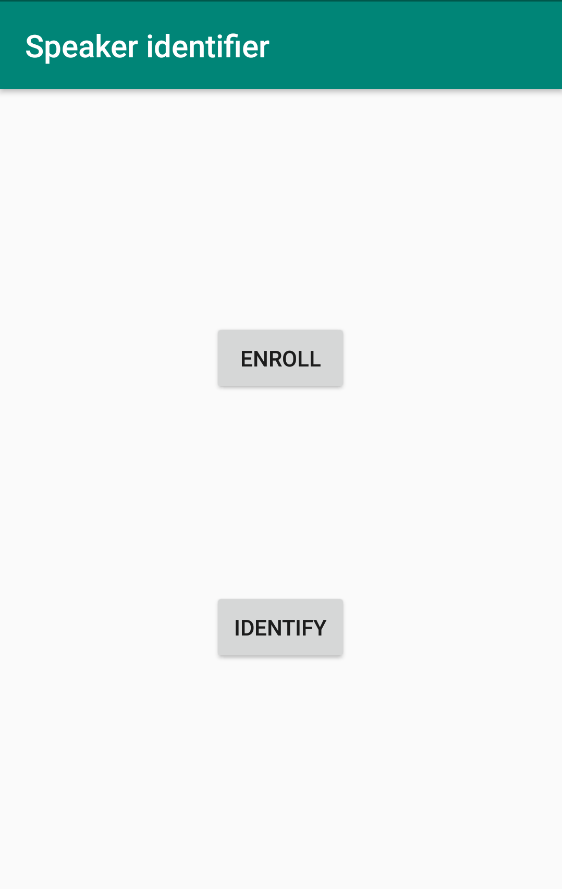
\includegraphics[width=40mm, keepaspectratio]{figures/app-main-screen.png}
	\caption{Menü.}
	\label{fig:app-main-screen}
\end{figure}

A regisztrációs felületen megadjuk a nevet, majd a \emph{Record} gombra kattintva három másodperc múlva elindul a hangfelvétel, ami négy másodpercen keresztül tart. A felületen megjelenő információ folyamatosan tájékoztatja a felhasználót a hangfelvétel folyamatáról.

\begin{figure}[!ht]
	\centering
	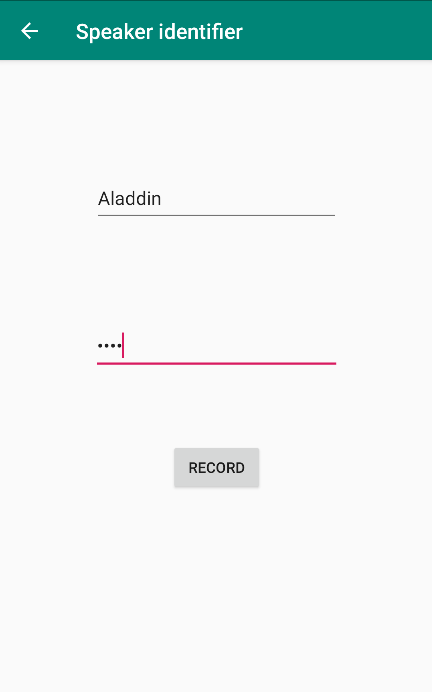
\includegraphics[width=40mm, keepaspectratio]{figures/app-register-screen-1.png}
	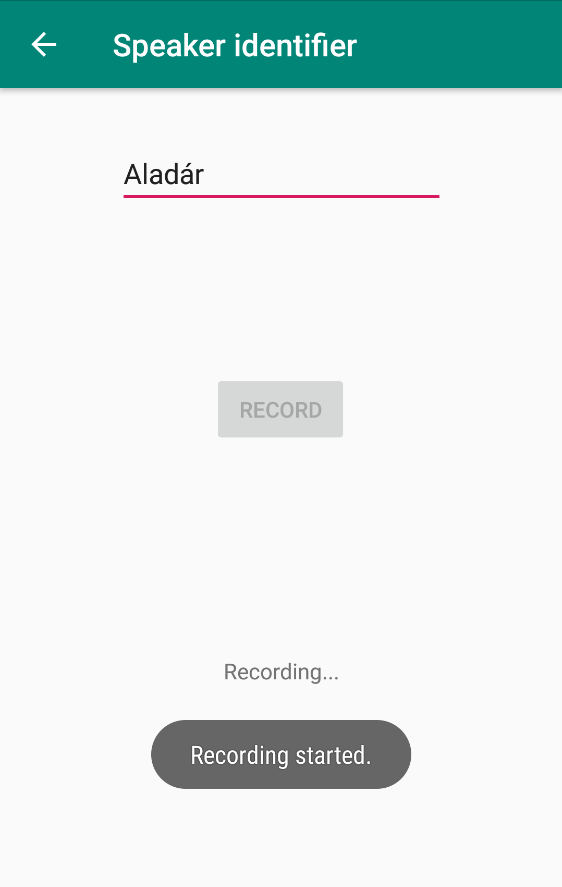
\includegraphics[width=40mm, keepaspectratio]{figures/app-register-screen-2.png}
	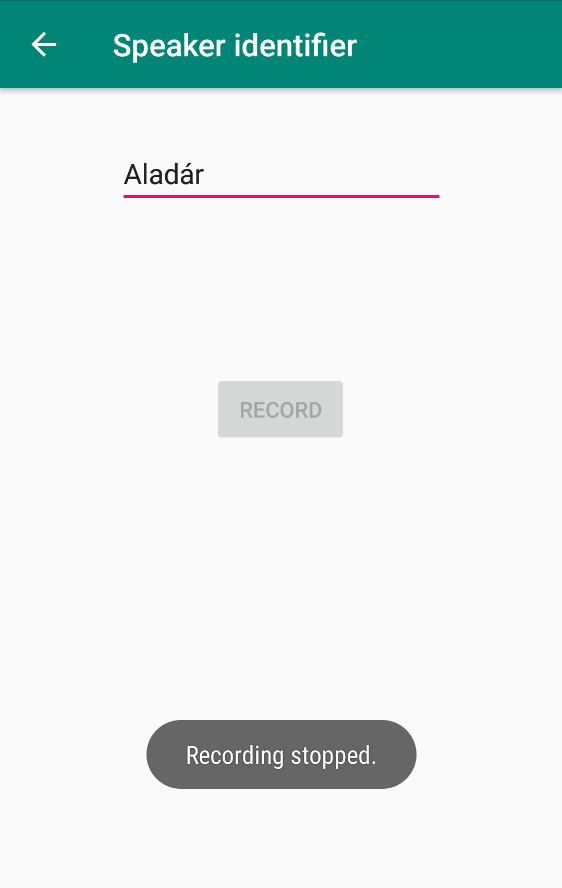
\includegraphics[width=40mm, keepaspectratio]{figures/app-register-screen-3.png}
	\caption{Felhasználói felület regisztrációhoz.}
	\label{fig:app-register-screen-1}
\end{figure}

A zöld fejlécen a vissza nyílra kattintva visszajutunk a főmenübe. Ezt az opciót a manifest fájlban a \emph{parentActivityName} tag megadásával érhetjük el.

\begin{figure}[!ht]
	\centering
	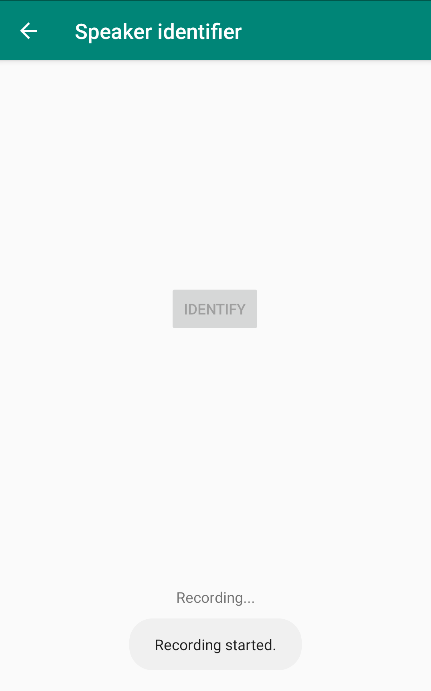
\includegraphics[width=40mm, keepaspectratio]{figures/app-identify-screen-1.png}
	\caption{Felhasználói felület azonosításhoz.}
	\label{fig:app-identify-screen-1}
\end{figure}

\newpage
A főmenüből az azonosító felületre lépve az \emph{Identify} gombra kattintva szintén visszaszámlálásra elindul a hangrögzítés, ami négy másodperig tart. Ezután megkapjuk a választ; az azonosított felhasználó nevét, vagy a nem sikerült azonosítani üzenetet.

\subsubsection{Osztálydiagram és részletes működés}

\begin{figure}[!ht]
	\centering
	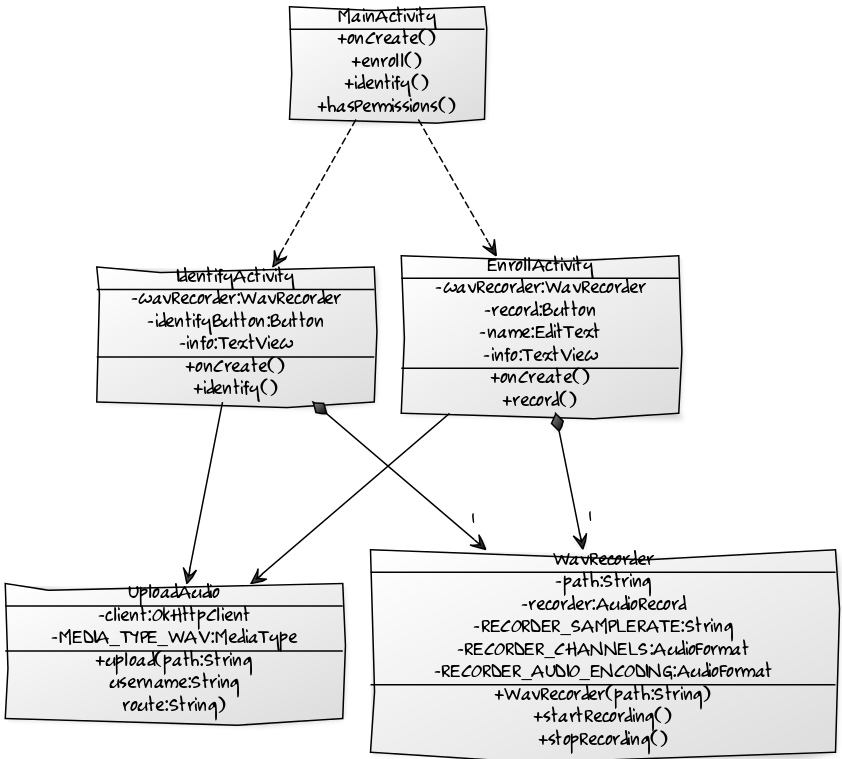
\includegraphics[width=130mm, keepaspectratio]{figures/app-class-diag.png}
	\caption{Beszélőfelismerő alkalmazás: Osztálydiagram.}
	\label{fig:app-class-diag}
\end{figure}

A \emph{MainActivity} osztály tartozik a főmenühöz. Amikor a főmenübe lépünk, az \emph{onCreate} metódus hívódik meg, amely ellenőrzi, hogy az alkalmazásnak megvannak-e a szükséges engedélyei a \emph{hasPermission} segédmetódus által. Ha igen akkor nem tesz semmit, egyébként a felhasználótól az összes engedély megadását kéri.

Az \emph{enroll} metódus a felületen az \emph{Enroll} gombhoz, az \emph{identify} az \emph{Identify} gombhoz tartozik. Mindkét függvény létrehoz egy-egy \emph{Intent}-et ami a hivatalos definíció szerint egy elvégzendő művelet absztrakt leírása. Az \emph{Intent} valójában arra jó, hogy egy felületről egy másik felületre lépjünk. A kiinduló felületen egy gombra kattintva (pl. \emph{Enroll}), a gombhoz tartozó listener metódus (\emph{enroll()}) hívódik meg, ami létrehoz egy \emph{Intentet} paraméterként átadva az elérni kívánt felülethez tartozó \emph{Activity} osztályt (\emph{EnrollActivity}). Ezután az \emph{Intentet} elindítva átlépünk a felületre.

A regisztrációs felületre lépve az \emph{onCreate} metódus meghívásakor az \emph{EnrollActivity} példányosít egy \emph{WavRecorder} objektumot a fájl elérési útjával paraméterezve. A \emph{record} metódus visszaszámlál, kiírja a felhasználónak az időzített üzeneteket, és elindítja majd megállítja a \emph{WavRecordert}.

Az időzítést az ajánlás szerint a \emph{Handler} osztály segítségével végeztem. Ennek előnye, hogy az időzített feladatokat egy háttérszálon futtatja, így nem blokkol. Így nem történhet meg, hogy egy hosszabb feladat elvégzése miatt a felületen nem kattinthatunk amíg az nincs kész.

Az \emph{IdentifyActivity} osztály nagyon hasonlóan működik. A különbség, hogy a \emph{EnrollActivity}-hez képest nem küld nevet és más címre küldi a hangfájlt.

Mindkét osztály a \emph{UploadAudio} objektumot használ a fájl szerverhez való elküldéséhez. Az \emph{UploadAudio} egy \emph{OkHttpClient} http klienst használ és \emph{multipart/form} Http POST kérést küld a szerver felé a hangfájllal ill. regisztrációkor a névvel. Ezután egy callback metódussal várja a szerver válaszát, amit az azonosító felületre továbbít.

\subsection{Szerver}

Szerver oldalon egy Flask python alkalmazás fut felhőben, és REST API-val rendelkezik. Fogadja a klienstől érkező hangfájlokat, előfeldolgozza és tárolja őket. Azonosításkor a modellen prediktál, majd visszaküldi az eredményt a kliensnek.

\subsubsection{Flask}

A Flask egy Python nyelvhez készült web mikrokeretrendszer. Mikrokeretrendszernek nevezzük a minimális webalkalmazás keretrendszereket, amelyekből általában hiányoznak a autentikációs, autorizációs könyvtárak, az objektum-relációs leképzés stb.

A Flask előnye, hogy nagyon gyorsan és könnyedén lehet vele REST API-t készíteni és elindítani a webalkalamzást. Nincs szükség más könyvtárakra, toolokra hozzá.

\subsubsection{Projekt felépítése}

\begin{itemize}
	\item \emph{app/app.py}: A webalkalmazást indító és a logikát tartalmazó (előfeldolgozás, predikció, fájlok kezelése) Python szkript.
	\item \emph{config.py}: Konfigurációs objektumokat tartalmaz.
	\item \emph{data}: Tartalmazza a klienstől regisztrációs és azonosítani kívánt \emph{wav} fájlokat és a preprocesszált állományokat.
	\item \emph{model}: A beszélőfelismerésre használt modelleket tároló mappa.
\end{itemize}

\subsubsection{Részletes működés}